% ---------------------------------------------------------------
% Preamble
% ---------------------------------------------------------------
%\documentclass[a4paper,fleqn,longmktitle]{cas-sc}
\documentclass[a4paper,fleqn]{cas-dc}
%\documentclass[a4paper]{cas-dc}
%\documentclass[a4paper]{cas-sc}
% ---------------------------------------------------------------
% Make margins bigger to fit annotations. Use 1, 2 and 3. TO be removed later
%\paperwidth=\dimexpr \paperwidth + 6cm\relax
%\oddsidemargin=\dimexpr\oddsidemargin + 3cm\relax
%\evensidemargin=\dimexpr\evensidemargin + 3cm\relax
%\marginparwidth=\dimexpr \marginparwidth + 3cm\relax
% -------------------------------------------------------------------- 
% Packages
% --------------------------------------------------------------------
% Figure packages
\usepackage{graphicx}
\usepackage{float}
\restylefloat{table}
\usepackage{adjustbox}
% Text, input, formatting, and language-related packages
\usepackage[T1]{fontenc}
\usepackage{subcaption}

\usepackage{csvsimple}

% TODO package
\usepackage[bordercolor=gray!20,backgroundcolor=blue!10,linecolor=black,textsize=footnotesize,textwidth=1in]{todonotes}
\setlength{\marginparwidth}{1in}
% \usepackage[utf8]{inputenc}
% \usepackage[nomath]{lmodern}

% Margin and formatting specifications
%\usepackage[authoryear]{natbib}
\usepackage[sort]{natbib}
\setcitestyle{square,numbers}

 %\bibliographystyle{cas-model2-names}

\usepackage{setspace}
\usepackage{subfiles} % Best loaded last in the preamble

% \usepackage[authoryear,longnamesfirst]{natbib}

% Math packages
\usepackage{amsmath, amsthm, amssymb, amsfonts, bm, nccmath, mathdots, mathtools, bigints, ulem}

\usepackage{tikz}
\usepackage{pgfplots}
\usetikzlibrary{shapes.geometric,angles,quotes,calc}

\usepackage{placeins}

\usepackage[final]{pdfpages}

\usepackage{numprint}

% --------------------------------------------------------------------
% Packages Configurations
\usepackage{enumitem}
% --------------------------------------------------------------------
% (General) General configurations and fixes
\AtBeginDocument{\setlength{\FullWidth}{\textwidth}}	% Solves els-cas caption positioning issue
\setlength{\parindent}{20pt}
%\doublespacing
% --------------------------------------------------------------------
% Other Definitions
% --------------------------------------------------------------------
\graphicspath{{Figures/}}
% --------------------------------------------------------------------
% Environments
% --------------------------------------------------------------------
% ...

% --------------------------------------------------------------------
% Commands
% --------------------------------------------------------------------

% ==============================================================
% ========================== DOCUMENT ==========================
% ==============================================================
\begin{document} 
%  --------------------------------------------------------------------

% ===================================================
% METADATA
% ===================================================
\title[mode=title]{Supercritical fluid extraction of essential oil from chamomile seeds: modelling, and parameter estimation}                      
\shorttitle{Supercritical fluid extraction of essential oil from chamomile seeds: modelling, and parameter estimation}

\shortauthors{OS, PO}

\author[1]{Oliwer Sliczniuk}[orcid=0000-0003-2593-5956]
\ead{oliwer.sliczniuk@aalto.fi}
\cormark[1]
\credit{a}

\author[1]{Pekka Oinas}[orcid=0000-0002-0183-5558]
\credit{b}

\address[1]{Aalto University, School of Chemical Engineering, Espoo, 02150, Finland}
%\address[2]{2}

\cortext[cor1]{Corresponding author}

% ===================================================
% ABSTRACT
% ===================================================
\begin{abstract}
This study investigated the supercritical extraction process of chamomile oil from chamomile seeds. A distributed-parameter model describes the fluid-solid extraction process. The concept of quasi-one-dimensional flow is applied to reduce the number of spatial dimensions. The flow is assumed to be uniform across any cross-section, although the area available for the fluid phase can vary along the extractor. The physical properties of the solvent are estimated from the Peng-Robinson equation of state. Key model parameters included partition factor internal and axial diffusion coefficients were determined using maximum likelihood estimation from experimental data, assuming normal error. A set of laboratory experiments was performed in under multiple constant operating conditions: $30 - 40^\circ C$, $100 - 200$ bar, and $3.33-6.67 \times 10^{-5}$ kg/s. 

\end{abstract}

\begin{keywords}
Supercritical extraction \sep Parameter estimation \sep Mathematical modelling
\end{keywords}

% ===================================================
% TITLE
% ===================================================
\maketitle

% ===================================================
% Section: Introduction
% ===================================================\section{Introduction}

\section{Introduction}
\subfile{Sections/introduction_imp}

\section{Materials and methods} \label{CH: Materials and methods}

\subsection{Supercritical fluids} \label{CH: Thermodynamic}
\subfile{Sections/Thermo_imp}

\subsection{Governing equations} \label{CH:Governing_equations_chapter}
	The governing equation for a quasi-one-dimensional compressible flow in Cartesian coordinates can be found in the Appendix \ref{CH: Gouverning equations} and in the work of \citet{Anderson1995}. Quasi-one-dimensional flow is a fluid flow characterized by the assumption that the flow properties remain uniform across any given cross-section of the flow. This assumption is made when there is a variation in the cross-sectional area of the flow channel, such as an irregular shape or partial filling of an extractor. In such cases, the flow is considered to be quasi-one-dimensional because the velocity and other flow properties are assumed to vary only in the direction of flow.

The quasi-one-dimensional compressible Navier-Stokes equations in Cartesian coordinates are given by Equations \ref{EQ: CompressibleEuler_1} to \ref{EQ: CompressibleEuler_3}. The derivation of these Equations are presented in Appendix \ref{CH: Gouverning equations}.

{\footnotesize
	\begin{align}
		\label{EQ: CompressibleEuler_1}
		\cfrac{\partial \left( {\color{black}\rho_f} {\color{black}A_f}(z) \right) }{\partial t} + \cfrac{\partial \left( {\color{black}\rho_f} {\color{black}A_f}(z) v \right)}{\partial z} &= 0 \\
		\cfrac{\partial \left( {\color{black}\rho_f} v {\color{black}A_f}(z) \right) }{\partial t} + \cfrac{\partial \left( {\color{black}\rho_f} {\color{black}A_f}(z) v^2 \right)}{\partial z} &= -{\color{black}A_f}(z) \cfrac{\partial {\color{black}P}}{\partial z} \label{EQ: CompressibleEuler_2} \\
		\cfrac{\partial \left( {\color{black}\rho_f} {\color{black}e} {\color{black}A_f}(z) \right) }{\partial t} + \cfrac{\partial \left( {\color{black}\rho_f} {\color{black}A_f}(z) v {\color{black}e}\right)}{\partial z} &= -{\color{black}P}\cfrac{\left( {\color{black}A_f}(z) v \right)}{\partial z} + \cfrac{\partial}{\partial z} \left( \cfrac{\partial {\color{black}T}}{\partial z} \right)   
		\label{EQ: CompressibleEuler_3}
	\end{align}  
}

where ${\color{black}\rho_f}$ is the density of the fluid, ${\color{black}A_f}(z)$ is the function which describe change of the cross-section, $v$ is the velocity, ${\color{black}P}$ is the total pressure, ${\color{black}e}$ is the internal energy of the fluid, $t$ is time and $z$ is the spacial direction.

Based on governing equations, the small discontinuity (defined as $\delta$) in flow properties, shown in Figure \ref{fig: Discontinuity_slow_flow}, can be analysed. The analysis follows the work of \citet{Schreier1982}.

\begin{figure}[!h]
	\centering
	\resizebox{0.95\columnwidth}{!}{%
		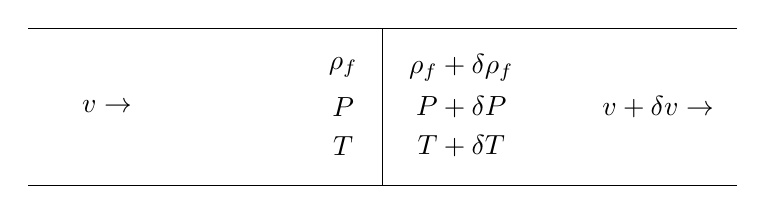
\begin{tikzpicture}[]
			\draw (0,2) -- (9,2);	% Top line
			\draw (0,0) -- (9,0); 	% Bottom line
			\draw (4.5,0) -- (4.5,2); 	% Bottom line
			\node at (4,1.5) {${\color{black}\rho_f}$};
			\node at (5.5,1.5) {${\color{black}\rho_f}+\delta{\color{black}\rho_f}$};
			\node at (4,1.0) {${\color{black}P}$};
			\node at (5.5,1.0) {${\color{black}P}+\delta {\color{black}P}$};
			\node at (4,0.5) {${\color{black}T}$};
			\node at (5.5,0.5) {${\color{black}T}+\delta {\color{black}T}$};
			\node at (1,1.0) {$v \rightarrow$};
			\node at (8,1.0) {$v + \delta v \rightarrow$};
	\end{tikzpicture} }
	\caption{Small discontinuity in one-dimensional flow}
	\label{fig: Discontinuity_slow_flow}
\end{figure} 

The discontinuity is presumed to be at rest relative, and the balance equations become		

{\footnotesize
	\begin{align*}
		&{\color{black}\rho_f} \delta v + v \delta {\color{black}\rho_f} + \delta {\color{black}\rho_f} \delta v = 0 \\
		&\delta {\color{black}P} = \delta v \delta {\color{black}\rho_f}
	\end{align*}
}

These relations are equally valid if the two regions are separated by a region of finite width rather than a discontinuity. 

{\footnotesize
	\begin{equation*}
		\lim_{{\color{black}\rho_f} v \rightarrow 0} {\color{black}\rho_f} \delta v + v \delta {\color{black}\rho_f} + \delta {\color{black}\rho_f} \delta v = 0 / \delta {\color{black}\rho_f} \rightarrow \cfrac{d v}{d {\color{black}\rho_f}} = - \cfrac{v}{{\color{black}\rho_f}}
	\end{equation*}
}

By combining the momentum equation with the above equation, we get

{\footnotesize
	\begin{equation} \label{EQ: Pressure_Velocity}
		\cfrac{d v}{d {\color{black}\rho_f}} = - \cfrac{d v}{d{\color{black}P}} \cfrac{d {\color{black}P}}{d {\color{black}\rho_f}} = -\cfrac{1}{\rho v} \cfrac{d{\color{black}P}}{d{\color{black}\rho_f}} = -\cfrac{v}{{\color{black}\rho_f}}
	\end{equation}
}

Suppose the flow is presumed to be isentropic, $d{\color{black}P}/d{\color{black}\rho_f} = c^2$, so $v^2=c^2$, where $c$ is the speed of sound. This can be interpreted as a small pressure wave propagating with the speed of sound relative to the flow. Moreover, if the flow velocity is relatively low, all pressure changes are hydrodynamic (due to velocity motion) rather than thermodynamic which leads to $\partial {\color{black}\rho_f} / \partial {\color{black}P} \approx 0$. In other words, the small changes in pressure due to flow velocity changes do not change the density. 

\subsection{Extraction model} \label{CH: Extraction_model}
\subfile{Sections/Model}

\subsection{Parameter estimation} \label{CH: Parameter_estimation}
\subfile{Sections/Parameter_estimation}

\subsection{Experimental work}
\subfile{Sections/Experiments}

\section{Results}
\subfile{Sections/Results_Chamomile}

\section{Conclusions} \label{CH: Conclusion}

%This study presented basic aspects regarding the laboratory work for obtaining chamomile extracts using supercritical carbon dioxide at different operating conditions. A first-principle process model was developed based on governing equations. As a result of the literature review, the extraction kinetic model was selected and combined with the general mass balance equations. The values of unknown parameters in the process model were obtained by parameter estimation. The yield data from the experiments were compared against the yield generated by the model. The IPOPT solver was used to solve the maximum likelihood estimation. The process model was found to have good agreement with experimental yield curves. Later, the parameters found for each experiment were combined to obtain more general relationships. The correlations for diffusion and decay coefficients are presented as a function of fluid density or Reynolds number. It should be noted that obtained correlations have been prepared with a limited amount of data. These correlations can be used to study qualitatively the impact of different operating conditions on the extraction yield by different methods, such as sensitivity analysis. Moreover, the generalized model could be useful in finding the optimal operating conditions with respect to the process economy.

% ===================================================
% Bibliography
% ===================================================
%% Loading bibliography style file
\clearpage
%\bibliographystyle{model1-num-names}
\bibliographystyle{unsrtnat}
\bibliography{mybibfile}

\clearpage \appendix \label{appendix}
\section{Appendix} 
\subsection{Thermodynamic}
\subfile{Sections/Qubic_EOS}

\subsection{Governing equations}
\subfile{Sections/Gouverning_equation_derivation}

\subsection{Cardano's Formula} \label{CH: Cardano}
\subfile{Sections/Cardano}

%\subsection{Initial and boundary conditions} \label{CH: IC_BC}
%\subfile{Sections/IC_BC}

\subsection{Maximum likelihood} \label{CH: ML}
\subfile{Sections/Likelihood}

%\subsection{Solid density measurement} \label{CH: Solid_Density_Measurment}

%Figure \ref{fig:density_cal} shows results of density measurement performed with pycnometer.

%\begin{figure}[!h]
%	\centering 
%	\includegraphics[trim=2cm 6cm 4cm 0cm, clip,width=\columnwidth]{Sections/ultraReportT5.pdf}
%	\caption{The result of solid density measurement}
%	\label{fig:density_cal}
%\end{figure}

%{\footnotesize
%	\begin{equation*}
%		\rho_s^{ave} = \frac{1.2585+1.2582+1.2561+1.2546+1.2555}{5} = 1.25658 [g/cc]
%	\end{equation*}
%}

%\subsection{Porosity calculations} \label{CH: Porosity}
%\subfile{Sections/Porosity}

\end{document}